\chapter{Introduction}
\label{introduction}

When looking at the recent trends in the car industry, autonomous driving is probably one of the most important topics. As Elon Musk founder of Tesla said ``I think that all cars will go fully autonomous in long-term. I think it will be quite unusual to see cars that don’t have full autonomy,'' autonomous driving will be the future of the car industry\cite{musk}.\\

This trend can also be seen in other industries  in which autonomous robots are used to simplify and accelerate production steps. 



The event ``Carolo-Cup'' hosted by the Technical University of Braunschweig offers a place for teams to compete against each other with their autonomous 1:10 model cars and therefore supports the development of the research field itself. This creates an incentive to participate to a lot of universities in Germany and beyond.\\
\todo{existing, goal and this work relations }

At the moment of the start of this work the existing part was solely the roadDetection developed by Prof. Dr.-Ing. Stefan Hörmann with the goal to use it in the Carolo-Cup. To use it, a software stack has to be build around it, that uses the data to navigate the robot on the course, the development of this stack is addressed in this thesis.


The navigation of a mobile system from ground up includes a wide range of topics and problems, such as sensor data filtering and combination to generate a stable and reliable odometry, or path finding in an environment including obstacles with respect to the dynamics of the robot.\\

Extending the work of Prof. Dr-Ing. Stefan Hörmann on his ROS based road detection, this navigation will also be developed for ROS Noetic. This allows the usage of various packages supplied as open source projects for the ROS framework.

\section{Structure}

This thesis is structured into four main parts, while Chapter \ref{theoretical_background} provides information about the needed theoretical knowledge.


Chapter \ref{Concept} covers the initial planning of the navigation in form of a concept. It incorporates initial approaches and gives a broad introduction to the structure of the navigation.\\

In chapter \ref{Selection} the selection of the nodes of the base structure of the stack is discussed. Furthermore the development of all custom nodes is covered

The configuration and test setup of the nodes in the stack is covered in chapter \ref{configurationandtesting}.


Finally the results of the tests are discussed in chapter \ref{resultanddiscussion}, which leads to potentially needed optimizations and a conclusion of the performance of the navigation.

\section{Limitations and requirements}

Before diving into the details and developing concepts the guidelines and requirements of the project have to be defined.

This thesis aims for a navigation of a robot in an environment that is similar to the Carolo-Cup but deviates at some parts.

\subsection{Robot and environment}
While the robot itself has very strict regulations in the Carolo-Cup these do not all apply here.\\

For testing purposes the entire robot with all sensors and the drive controller are simulated.

The robot used in this thesis is a differential drive robot from the company Parallax with a diameter of 450mm as pictured in Figure \ref{arlore}.\\

\begin{figure}[H]
	\centering
	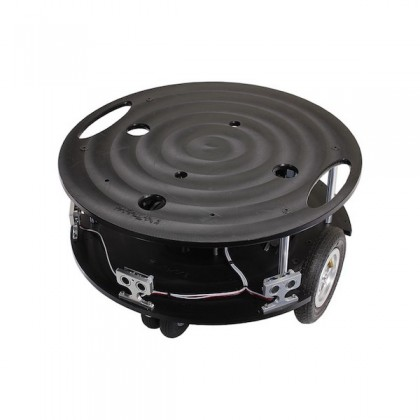
\includegraphics[width=.7\textwidth]{arlo real}
	
	\caption{Mobile robot Parallax Arlo \cite{arloreal}}
	\label{arlore}
\end{figure}


Equally to the Carolo-Cup regulations the lane width is defined by double robot width and therefore 900 mm. 

The robot is equipped with the following sensors:

\begin{itemize}
	\item Lidar
	\item Wheel encoder
	\item IMU
	\item Camera
\end{itemize}

Additional it features a motor driver for differential drive steering.

\section{Software}
Generally the software is developed for ROS-Noetic.\\
The programming language is mostly C++ to allow uniformity in the software stack.\\
Like in the Carolo-Cup the software is not supposed to have any connection to systems outside of the robot.\\

\subsection{Simulation}
Since the environment is simulated the simulator has to have the following features.
\begin{itemize}
	\item Sensor plugins with configurable error and ROS interfaces
	\item Differential drive plugin
	\item Custom models integration
	\item URDF conversion
	\item Not too computationally heavy
\end{itemize}

The simulation is mostly focus on sensor data. That is why sensor plugins with configurable error and a ROS interfaces are needed. Like this the data will be as representative as possible of the real world.\\

In addition to the sensor plugins the simulator needs to provide a plugin for differential drive steering. This is the replacement for the motor controller of the real robot.\\

Custom models is a strict requirement since this thesis focuses on a very specific robot. Furthermore the integration of custom models is necessary to put the robot in different road scenarios.\\

A URDF conversion plugin is very important like this differences between the simulated robot and the tf-tree in ROS can be avoided and the robot will be defined in one file only.\\

To get the best correlation between simulation and real world, the simulator should be able to run close to real time. This will make the simulated sensor data way more reliable and puts the nodes of the navigation\_stack under a realistic load.

\subsection{Navigation}
The navigation is supposed to cover free driving without obstacles, as well as with static obstacles avoidance. It will not cover dynamic obstacles, road sign detection or driving situations like intersections and parking.\\

Development of an entire stack exceeds the content of this thesis, so an open source navigation project will be used which needs to satisfy the following requirements.

\begin{itemize}
	\item Sensor input.
	\item Goal pose input
	\item 2D mobile platform support usage of the conventional drive systems like ackermann and differential
	\item Path planning in respect to the robots kinematic and shape, as well as the environment detected by the sensors.
	\item Path planning and navigation in totally unknown environments
	\item Velocity output as linear and angular velocities
\end{itemize}

\todo{beschreibung}
